% file: graph-paths/bitonic-path.tex

\documentclass[tikz]{standalone}

\usetikzlibrary{positioning, decorations.pathmorphing}

\begin{document}
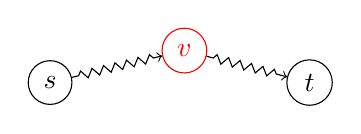
\begin{tikzpicture}[n/.style = {circle, draw}, % node
    leadsto/.style = {->, decorate, decoration = {
    	zigzag, amplitude = 1.50pt, segment length = 1.5mm, pre length = 2.5pt, post length = 2.5pt}},
    e/.style = {->}, % edge
  ]
  \node (s) [n] {$s$};

  \node (v) [n, above right = 0.2cm and 1.5cm of s.center, red] {$v$};
  \node (t) [n, right = 3.0cm of s.center] {$t$};

  \path (s) edge[leadsto] (v)
	(v) edge[leadsto] (t);
\end{tikzpicture}
\end{document}
